
\de{ĐỀ THI GIỮA HỌC KỲ I NĂM HỌC 2022-2023}{THPT Tân Bình}

\Opensolutionfile{ans}[ans/TanBinh-HCM-TNTL]
%%==========Câu 1
\begin{ex}%[0D1Y1-2]%[Dự án đề kiểm tra HK1 22-23-Nhật Thiện]%[Trường Tân Bình]
Mệnh đề nào sau đây đúng?
\choice
{$0=\{0\}$}
{$0=\varnothing$}
{\True $0 \in\{0\}$}
{$0 \subset\{0\}$}
 \loigiai{
Ta có $0 \in\{0\}$.
}
\end{ex}
%%==========Câu 2
\begin{ex}%[0H5Y1-3]%[Dự án đề kiểm tra HK1 22-23-Nhật Thiện]%[Trường Tân Bình]
Cho hình bình hành $MNPQ$. Véc-tơ nào bằng với $\vec{MN}$?
\choice
{$\vec{PQ}$}
{\True $\overrightarrow{QP}$}
{$\overrightarrow{MP}$}
{$\vec{NP}$}
\loigiai{
\immini{Ta có $\vec{MN}=\vec{QP}$.}
{\begin{tikzpicture}[>=stealth,x=1cm,y=1cm,scale=1, font=\footnotesize] 
	\foreach \vitrinhandiem/\diem/\x/\y in {below/M/0/0,below/N/4/0,above/P/6/2,above/Q/2/2}	
	\coordinate[label=\vitrinhandiem:$\diem$] (\diem) at (\x,\y);
	\draw (M)--(N)--(P)--(Q)--(M);
\end{tikzpicture}}
}
\end{ex}
%%==========Câu 3
\begin{ex}%[0H4Y1-1]%[Dự án đề kiểm tra HK1 22-23-Nhật Thiện]%[Trường Tân Bình]
Cho góc $\alpha$ là góc tù. Khẳng định nào sau đây là đúng?
\choice
{\True $\cot \alpha<0$}
{$\cos \alpha>0$}
{$\sin \alpha<0$}
{$\tan \alpha>0$}
\loigiai{
Do $\alpha$ là góc tù nên $\cot \alpha<0$.
}
\end{ex}
%%==========Câu 4
\begin{ex}%[0D1Y1-4]%[Dự án đề kiểm tra HK1 22-23-Nhật Thiện]%[Trường Tân Bình]
Biết rằng $P\Rightarrow Q$ là mệnh đề đúng. Mệnh đề nào sau đây đúng?
\choice
{$Q$ là điều kiện cần và đủ để có $P$}
{$Q$ là điều kiện đủ để có $P$}
{\True $P$ là điều kiện đủ để có $Q$}
{$P$ là điều kiện cần để có $Q$}
\loigiai{
Mệnh đề $P\Rightarrow Q$ được phát biểu là \lq\lq$P$ là điều kiện đủ để có $Q$\rq\rq.
}
\end{ex}
%%==========Câu 5
\begin{ex}%[0D2Y1-1]%[Dự án đề kiểm tra HK1 22-23-Nhật Thiện]%[Trường Tân Bình]
Trong các bất phương trình sau, bất phương trình nào \textbf{không phải} là bất phương trình bậc nhất hai ẩn?
\choice
{$2 x-3 y \leq 2022$}
{$x+2022>0$}
{\True $\dfrac{x}{y}+1>0$}
{$5 x+y \geq 2 x+11$}
\loigiai{
Bất phương trình $\dfrac{x}{y}+1>0$ không phải là bất phương trình bậc nhất hai ẩn.
}
\end{ex}
%%==========Câu 6
\begin{ex}%[0D3B1-4]%[Dự án đề kiểm tra HK1 22-23-Nhật Thiện]%[Trường Tân Bình]
Cho hàm số $y=f(x)$ có đồ thị hàm số như hình bên dưới. Hàm số đồng biến trên khoảng nào sau đây?
\begin{center}
	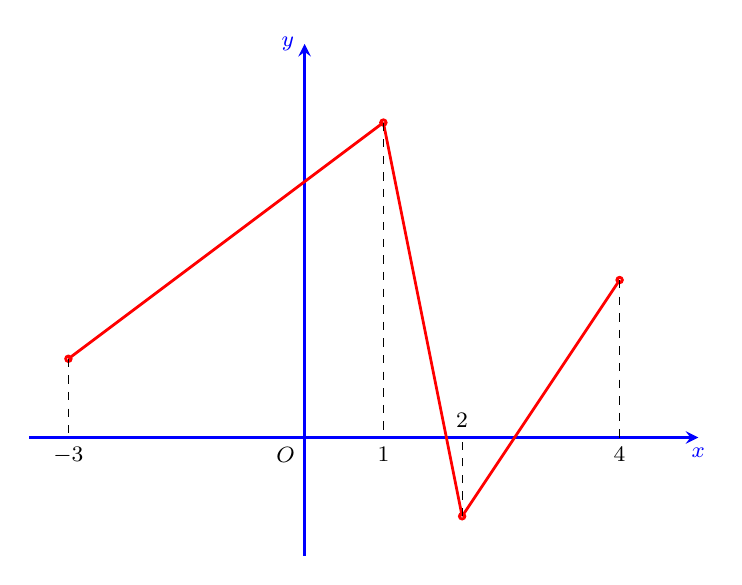
\begin{tikzpicture}[>=stealth,x=1cm,y=1cm,scale=1, font=\footnotesize] 
	\draw[blue, line width=1,->] (-3.5,0) -- (5,0) node[below] {$x$};
	\draw[blue, line width=1,->] (0,-1.5) -- (0,5) node[left] {$y$};
	\coordinate[label=below left:$O$] (O) at (0,0);
	\draw[red, line width=1] (-3,1)circle(1pt)--(1,4)circle(1pt)--(2,-1)circle(1pt)--(4,2)circle(1pt);
	\draw[dashed] (-3,1)--(-3,0)node[below]{$-3$} (1,4)--(1,0)node[below]{$1$} (2,-1)--(2,0)node[above]{$2$} (4,2)--(4,0)node[below]{$4$};
	\end{tikzpicture}
\end{center}
\choice
{\True $(-3 ; 1)$}
{$(-3 ; 4)$}
{$(2 ; 5)$}
{$(1 ; 2)$}
\loigiai{
Hàm số $y=f(x)$ có tập xác định $\mathscr{D}=[-3;4]$.\\
Dựa vào hình vẽ, ta có hàm số đồng biến trên khoảng $(-3;1)$.
}
\end{ex}
%%==========Câu 7
\begin{ex}%[0H5B2-1]%[Dự án đề kiểm tra HK1 22-23-Nhật Thiện]%[Trường Tân Bình]
Cho ba điểm $A$, $B$, $C$ phân biệt. Khẳng định nào sau đây đúng?
\choice
{\True $\overrightarrow{AB}+\overrightarrow{CA}=\overrightarrow{CB}$}
{$\vec{AB}+\vec{AC}=\vec{BC}$}
{$\overrightarrow{CA}-\overrightarrow{BA}=\overrightarrow{BC}$}
{$\overrightarrow{AB}-\overrightarrow{BC}=\overrightarrow{CA}$}
\loigiai{
Ta có $\overrightarrow{AB}+\overrightarrow{CA}=\overrightarrow{CA}+\overrightarrow{AB}=\overrightarrow{CB}$.
}
\end{ex}
%%==========Câu 8
\begin{ex}%[0D1Y3-1]%[Dự án đề kiểm tra HK1 22-23-Nhật Thiện]%[Trường Tân Bình]
Cho hai tập hợp $A=\{a; b; c; 1;2\}$ và $B=\{a; c; d; 1;3;5\}$. Khi đó tập $A\cup B$ có bao nhiêu phần tử?
\choice
{$6$}
{$11$}
{$3$}
{\True$8$}
\loigiai{
Ta có $A\cup B=\{a;b;c;d;1;2;3;5\}$. Do đó $A\cup B$ có $8$ phần tử.
}
\end{ex}
%%==========Câu 9
\begin{ex}%[0H4Y3-1]%[Dự án đề kiểm tra HK1 22-23-Nhật Thiện]%[Trường Tân Bình]
Cho tam giác $A B C$ với các cạnh $AB=c$, $AC=b$, $ BC=a$. Chọn công thức đúng trong các công thức sau
\choice
{$S=\dfrac{1}{2} ac \cdot \sin A$}
{\True $S=\dfrac{1}{2}bc \cdot\sin A$}
{$S=\dfrac{1}{2} bc \cdot \sin C$}
{$S=\dfrac{1}{2} bc \cdot \sin B$}
\loigiai{
Tam giác $A B C$ với các cạnh $AB=c$, $AC=b$, $ BC=a$. Khi đó $S=\dfrac{1}{2}bc \cdot\sin A$.
}
\end{ex}
%%==========Câu 10
\begin{ex}%[0D1Y3-2]%[Dự án đề kiểm tra HK1 22-23-Nhật Thiện]%[Trường Tân Bình]
Cho $A=\{-2 ;-1 ; 0 ; 1 ; 2\}$, $B=(-\infty ; 1]$. Tập hợp $A \setminus B$ bằng
\choice
{\True $\{2\}$}
{$\{-2 ;-1\}$}
{$\{-1\}$}
{$\{0 ; 1 ; 2\}$}
\loigiai{
Ta có $A \setminus B=\{2\}$.
}
\end{ex}
\Closesolutionfile{ans}
\begin{center}
	\textbf{PHẦN 2 - TỰ LUẬN}
\end{center}
%%==========Bài 1
\begin{bt}[1 điểm]%[0D1B3-4]%[Dự án đề kiểm tra HK1 22-23-Nhật Thiện]%[Trường Tân Bình]
Cho hai tập hợp $A=[-1;3]$ và $B=[0;5)$. Tìm $A\cap B$ và $A\setminus B$.
\loigiai{
Ta có $A\cap B=[0;3]$ và $A\setminus B=[-1;0)$.
}
\end{bt}
%%==========Bài 2
\begin{bt}[1 điểm]%[0D3B1-4]%[Dự án đề kiểm tra HK1 22-23-Nhật Thiện]%[Trường Tân Bình]
Xét tính đồng biến và nghịch biến của hàm số $f(x)=\dfrac{2}{x-3}$ trên khoảng $(3;+\infty)$.
\loigiai{
Tập xác định $\mathscr{D}=\mathbb{R}\setminus \{3\}$.\\
Lấy tùy ý $x_1,x_2 \in (3;+\infty)$ sao cho $x_1<x_2$, ta có
\begin{center}
	$x_1<x_2\Rightarrow x_1-3<x_2-3\Rightarrow \dfrac{2}{x_1-3}>\dfrac{2}{x_2-3}\Rightarrow f(x_1)>f(x_2)$.
\end{center}
Vậy hàm số nghịch biến trên khoảng $(3;+\infty)$.
}
\end{bt}
%%==========Bài 3
\begin{bt}[1 điểm]%[0H4B3-1]%[Dự án đề kiểm tra HK1 22-23-Nhật Thiện]%[Trường Tân Bình]
Cho tam giác $ABC$ có cạnh $a=2\sqrt{3}$\,cm, $b=2$\,cm, $\widehat{C}=30^\circ$. Tính diện tích tam giác $ABC$ và đường kính đường tròn ngoại tiếp tam giác $ABC$.
\loigiai{ 
\immini{Diện tích tam giác $ABC$ là \\
	$S=\dfrac{1}{2}ab\cdot\sin C=\dfrac{1}{2}\cdot 2\sqrt{3}\cdot 2\cdot\sin 30^\circ=\sqrt{3}$\,cm$^2$.\\
Áp dụng định lí cô-sin cho tam giác $ABC$, ta có
\allowdisplaybreaks
\begin{eqnarray*}
	c=AB&=& \sqrt{AC^2+BC^2-2\cdot AC\cdot BC\cdot\cos C} \\
	&=& \sqrt{2^2+(2\sqrt{3})^2-2\cdot 2\cdot 2\sqrt{3}\cdot\cos 30^\circ}= 2\,\text{cm}.
\end{eqnarray*}
Ta có $S=\dfrac{abc}{4R}\Rightarrow R=\dfrac{abc}{4S}=\dfrac{2\sqrt{2}\cdot 2\cdot 2}{4\cdot \sqrt{3}}=\dfrac{2\sqrt{6}}{3}$\,cm.}
{\begin{tikzpicture}[>=stealth,x=1cm,y=1cm,scale=1, font=\footnotesize] 
	\coordinate[label=below:$A$] (A) at (0,0);
	\pgfmathsetmacro\b{sqrt(3)}
	\coordinate[label=below:$C$] (C) at (2,0);
	\coordinate[label=above:$B$] (B) at ($(C)!\b!-30:(A)$);
	\draw (A)--(B)--(C)node[pos=0.5,above right]{$2\sqrt{3}$\,cm}--(A)node[pos=0.5,below]{$2$\,cm};
	\foreach \diem in {A,B,C}	\fill (\diem)circle(1pt);
	\draw pic["$30^{\circ}$", draw=blue, angle eccentricity=1.6, angle radius=0.5cm]{angle=B--C--A};
\end{tikzpicture}}
}
\end{bt}
%%==========Bài 4
\begin{bt}[1 điểm]%[0D2G2-2]%[Dự án đề kiểm tra HK1 22-23-Nhật Thiện]%[Trường Tân Bình]
Cho biết $226$\,g thịt bò chứa khoảng $59$\,g protein, Một quả trứng nặng $46$\,g có chứa khoảng $6$\,g (nguồn bộ nông nghiệp Hoa Kỳ). Giả sử có một người mỗi ngày cần không quá $60$\,g protein. Gọi số gam thịt bò và số gam trứng mà người đó ăn một ngày lần lượt là $x$, $y$.
\begin{enumerate}[a)]
	\item Lập bất phương trình theo $x$, $y$ diễn tả giới hạn về lượng protein mà người đó cần dùng mỗi ngày.
	\item Nếu người đó ăn $150$\,g thịt bò và $2$ quả trứng mỗi quả $46$\,g trong một ngày thì có phù hợp không?
\end{enumerate}
\loigiai{
\begin{enumerate}[a)]
	\item Ta có số gam thịt bò và số gam trứng mà người đó ăn trong một ngày là $x$, $y$.\\
	Do $226$\,g thịt bò chứa khoảng $59$\,g protein nên $x$\,(g) thịt bò chứa khoảng $\dfrac{59}{226}x$\,(g) protein.\\
	Do một quả trứng nặng $46$\,g có chứa khoảng $6$\,g nên $y$\,(g) trứng chứa khoảng $\dfrac{3}{23}y$\,(g) protein.\\
	Một người mỗi ngày cần không quá $60$\,g protein	nên ta có bất phương trình
	\begin{center}
	$\dfrac{59}{226}x+\dfrac{3}{23}y\le 60$.
	\end{center}
\item Người đó ăn $150$\,g thịt bò và $2$ quả trứng mỗi quả $46$\,g trong một ngày tương ứng với $x=150$ và $y=2\cdot 46=92$, thay vào bất phương trình, ta được
\begin{center}
	$\dfrac{59}{226}\cdot 150+\dfrac{3}{23}\cdot 92\le 60\Leftrightarrow \dfrac{5781}{113}\le 60$.
\end{center}
Đây là một mệnh đề đúng. Do đó, người này ăn $150$\,g thịt bò và $2$ quả trứng mỗi quả $46$\,g trong một ngày là phù hợp.
\end{enumerate}
}
\end{bt}
%%==========Bài 5
\begin{bt}[1 điểm]%[0H4G2-1]%[Dự án đề kiểm tra HK1 22-23-Nhật Thiện]%[Trường Tân Bình]
Hai máy bay cùng rời sân bay Tân Sơn Nhất cùng một lúc. Một chiếc máy bay với vận tốc $800$\,km/h hướng lệnh với hướng Bắc $15^\circ$ về phía Tây. Chiếc còn lại bay theo hướng lệch so mới hướng Nam về phía Tây với vận tốc $600$\,km/h. Hỏi hai máy bay đó cách nhau bao xa sau $3$ giờ bay? Giả sử chúng bay ở cùng một độ cao.
\begin{center}
	\begin{tikzpicture}[>=stealth,x=1cm,y=1cm,scale=1, font=\footnotesize] 
	\coordinate[label=above:Bắc] (B) at (0,3);
	\coordinate[label=below:Nam] (N) at (0,-3);
	\coordinate[label=right:Đông] (D) at (3,0);
	\coordinate[label=left:Tây] (T) at (-3,0);
	\coordinate[label=above right:$O$] (O) at (0,0);
	\coordinate (M) at ($(O)!0.8!15:(B)$);
	\coordinate (Q) at ($(O)!0.5!-135:(D)$);
	\draw[blue,line width=1pt,<->] (N)--(B);
	\draw[blue,line width=1pt,<->] (D)--(T);
	\draw[red,line width=1pt,->] (O)--(M)node[left]{$800$\,km/h};
	\draw[green!70!black,line width=1pt,->] (O)--(Q)node[below]{$600$\,km/h};
	\end{tikzpicture}
\end{center}
\loigiai{
Sau $3$ tiếng, chiếc máy bay với vận tốc $800$\,km/h hướng lệnh với hướng Bắc $15^\circ$ về phía Tây bay được $3\cdot 800=2\,400$\,(km).\\
Sau $3$ tiếng, chiếc còn lại bay theo hướng lệch so mới hướng Nam về phía Tây với vận tốc $600$\,km/h bay được $3\cdot 600=1\,800$\,(km).\\
Minh họa bằng hình vẽ.
\begin{center}
	\begin{tikzpicture}[>=stealth,x=1cm,y=1cm,scale=1, font=\footnotesize] 
	\coordinate (B) at (0,3);
	\coordinate (N) at (0,-3);
	\coordinate (D) at (3,0);
	\coordinate (T) at (-3,0);
	\coordinate[label=above right:$O$] (O) at (0,0);
	\coordinate[label=above:$M$] (M) at ($(O)!0.8!15:(B)$);
	\coordinate[label=below:$Q$] (Q) at ($(O)!0.5!-135:(D)$);
	\draw[blue,dashed] (N)--(B);
	\draw[blue,dashed] (D)--(T);
	\draw[red,line width=1pt,->] (O)--(M);
	\draw[green!70!black,line width=1pt,->] (O)--(Q);
	\draw (M)--(Q);
	\draw pic["$75^{\circ}$", draw=blue, angle eccentricity=1.6, angle radius=0.4cm]{angle=M--O--T};
	\draw pic["$45^{\circ}$", draw=blue, angle eccentricity=1.6, angle radius=0.45cm,double]{angle=T--O--Q};
	\end{tikzpicture}
\end{center}
Dựa vào dữ kiện bài toán, ta có $OM=2400$, $OQ=1800$ và $\widehat{MOQ}=75^\circ +45^\circ=120^\circ$.\\
Áp dụng định lí côsin cho tam giác $MOQ$, ta có 
\begin{eqnarray*}
	MQ&=& \sqrt{OM^2+OQ^2-2\cdot OM\cdot OQ\cdot\cos \widehat{MOQ}} \\
	&=& \sqrt{2400^2+1800^2-2\cdot 2400\cdot 1800\cdot\cos 120^\circ}\approx 3650.
\end{eqnarray*}
Vậy sau 3 giờ bay, hai máy bay cách nhau khoảng $3650$\,km.
}
\end{bt}
%%==========Bài 6
\begin{bt}[1 điểm]%[0D3G1-2]%[Dự án đề kiểm tra HK1 22-23-Nhật Thiện]%[Trường Tân Bình]
Tìm tất cả các giá trị thực của tham số $m$ để hàm số $y=\dfrac{\sqrt{3x+5m+6}}{x+m-1}$ xác định trên khoảng $(0;+\infty)$.
\loigiai{
Hàm số xác định trên khoảng $(0;+\infty)$ khi và chỉ khi
\allowdisplaybreaks
\begin{eqnarray*}
	\heva{&3x+5m+6\ge 0\\& x+m-1\ne 0},\forall x\in (0;+\infty) &\Leftrightarrow&  \heva{&m\ge \dfrac{-3x-6}{5}\\& 1-m\ne x},\forall x\in (0;+\infty)\\
	&\Leftrightarrow&  \heva{&m\ge \dfrac{-6}{5}\\& 1-m\le 0}\\
	&\Leftrightarrow&\heva{&m\ge \dfrac{-6}{5}\\& m\ge 1} \\
	&\Leftrightarrow& m\ge 1.
\end{eqnarray*}
Vậy $m\ge 1$.
}
\end{bt}